\chapter{THỰC NGHIỆM}
\label{Chapter4}

\section{Tập dữ liệu}

\setcounter{figure}{12}
\begin{figure}
	\centering
	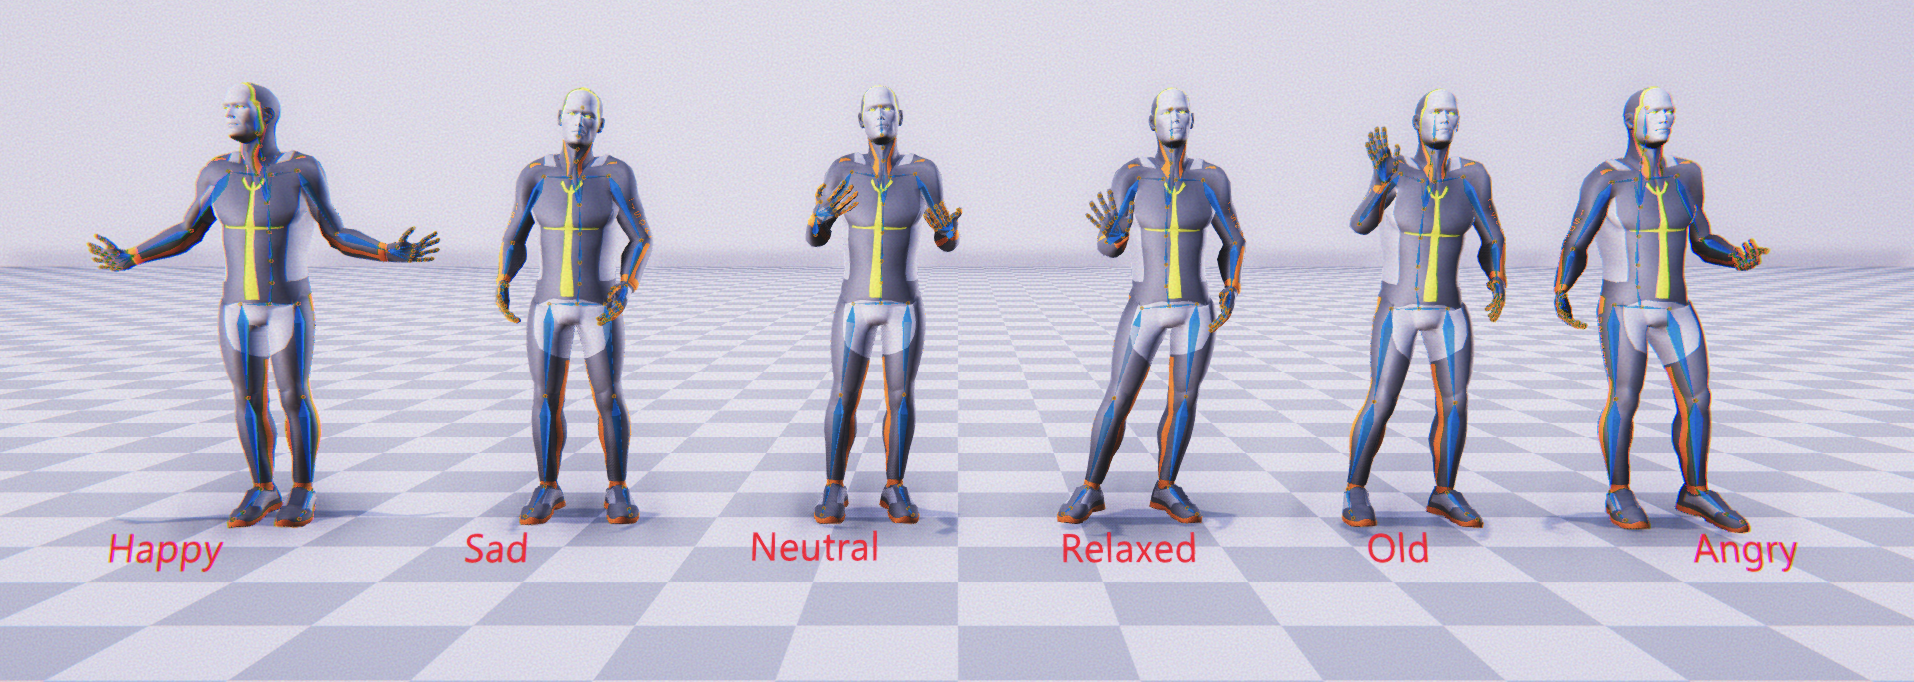
\includegraphics[width=\textwidth]{EmotionAnimation}
	\caption{Minh hoạ về 6 cử chỉ $\texttt{Happy}$, $\texttt{Sad}$, $\texttt{Neutral}$, $\texttt{Old}$, $\texttt{Relaxed}$ và $\texttt{Angry}$}
\end{figure}

Chúng tôi sử dụng tập dữ liệu ZeroEGGS \cite{ghorbani2022zeroeggszeroshotexamplebasedgesture} là một bộ dữ liệu motion capture được xây dựng để nghiên cứu và phát triển các mô hình tạo cử chỉ. Nó bao gồm 67 đoạn độc thoại do diễn viên motion capture nữ thực hiện, với tổng thời gian là 135 phút. Các đoạn hội thoại trong tập dữ liệu được biểu diễn với 6 cảm xúc khác nhau: $\texttt{Happy}$, $\texttt{Sad}$, $\texttt{Neutral}$, $\texttt{Old}$, $\texttt{Relaxed}$ và $\texttt{Angry}$, giúp mô phỏng nhiều trạng thái cảm xúc khác nhau trong cử chỉ và chuyển động cơ thể. ZeroEGGS cung cấp một nền tảng phong phú để nghiên cứu khả năng kết hợp giữa bài nói và cử chỉ động, phục vụ cho việc tạo ra các mô hình có thể điều chỉnh cử chỉ tương ứng với cảm xúc và ngữ nghĩa của văn bản.

\section{Quá trình xử lý dữ liệu}

Dữ liệu chúng tôi bao gồm các tệp tin BVH (BioVision Motion Capture) được thu nhận từ các cảm biến bằng các hệ thống Motion Capture. 


\textbf{Hierachy}: bao gồm 75 Bone $\{ \mathbf{t}_i \}^{75} $, có vị trí ban đầu  $\mathbf{t}_{i} = \{t_x, t_y, t_z\}$


\vspace{5pt}


\textbf{Motion}:
Bone trong dữ liệu BVH bao gồm vị trí $\mathbf{position}_{\operatorname{local}}  \in \mathbb{R}^{3}$ và góc quay $\mathbf{rotation}_{\operatorname{local}} \in \mathbb{R}^{3}$.

Chúng tôi chuyển dữ liệu từ góc quay Euler sang góc quay Quaternion, với góc quay Quaternion là một số phức gồm 3 số phức. 

Quá trình này được trình bày ở phụ lục \ref{Appendix2}

\section{Quá trình huấn luyện}

Toàn bộ quá trình huấn luyện mô hình được thực hiện trong vòng 1 ngày với các tham số sau: số bước huấn luyện $T = 1000$, sử dụng GPU Nvidia 3090, và chia tập dữ liệu theo tỷ lệ $8:1:1$ cho các tập training, testing và validation. Learning rate được thiết lập là $3 \times 10^{-5}$, với batch size là 384 và tổng cộng 300,000 mẫu. Quá trình huấn luyện được triển khai trên mã nguồn chương trình có sẵn tại: \hyperlink{https://github.com/hmthanh/OHGesture}{hmthanh/OHGesture} .


\section{Quá trình sử dụng Unity để kết xuất}

Để trực quan hóa quá trình sinh cử chỉ từ dữ liệu đầu ra của mô hình, chúng tôi sử dụng Unity, kết thừa mã nguồn từ mô hình DeepPhase \cite{starke2022deepphase}  . Dữ liệu sau khi sinh là file BVH (BioVision Motion Capture), trong Unity chúng tôi bổ sung mã nguồn CSharp để kết xuất theo vị trí toạ độ và nhãn tương ứng, với vị trí và góc quay của các xương được biểu diễn dưới dạng quaternion.

Chi tiết phần render cử chỉ được sinh ra, tôi trình bày ở phụ lục \ref{Appendix3}.

Mã nguồn chương trình Unity được chúng tôi công khai ở \hyperlink{https://github.com/DeepGesture/deepgesture-unity}{DeepGesture/DeepGesture-Unity}